\documentclass[11pt]{article}

\usepackage[margin=1in]{geometry}
\usepackage{amsmath,amssymb}
\usepackage{graphicx}

% plain-text stand-in for \url{} so the paper needs no hyperref/url package.
\newcommand{\url}[1]{\texttt{#1}}

% booktabs-style rules using only base LaTeX, for portability (no extra packages required)
\newcommand{\toprule}{\hline\hline}
\newcommand{\midrule}{\hline}
\newcommand{\bottomrule}{\hline\hline}

\title{The Engram as Hash, the Readout as Separation Operator:\\
Testing Two Recent Theories of Content-Addressable Memory}

\author{Gourav}

\date{\today}

\begin{document}
\maketitle

\begin{abstract}
We report two direct empirical tests of recent theoretical claims about content-addressable,
hippocampal-style memory, using a controlled testbed in which solved Sudoku grids are stored
as sparse binary engrams: each grid's $81\times81$ same-digit coincidence matrix is projected
through a fixed random sparse matrix and sparsified by $k$-winner-take-all, then retrieved
through an attention-style key-value readout. First, we test whether this encoder --
structurally identical to the random-projection-plus-winner-take-all circuit identified in the
fly olfactory mushroom body -- actually behaves as a similarity-preserving hash, rather than
assuming the analogy by construction. Across $390$ systematically corrupted queries spanning
the full corruption range, engram overlap with the true stored code tracks input similarity
almost monotonically (Spearman $\rho=0.974$, $p<10^{-250}$), and the floor of that relationship
lands almost exactly on the chance overlap predicted from code geometry alone ($K/H$), ruling
out a leftover-correlation artifact. Second, we test a very recent proposal that classical
correlation-matrix memory, sparse distributed memory, dense associative memory, and
Transformer-style attention are the same key-value computation, differing only in a
``separation operator'' nonlinearity applied to key-query similarity, by swapping our
readout's operator across all four families under a fully paired noise sweep on the identical
stored engrams and identical corrupted queries. The results both confirm and refine the
unification: some separating nonlinearity is a strict requirement for retrieval to function at
all among many competing memories (linear reweighting fails even with a noiseless query), but
robustness does not track how aggressively an operator discriminates -- it tracks whether the
operator sharpens by an absolute similarity \emph{gap} or a similarity \emph{ratio}.
Ratio-based sharpening (a rectified-power nonlinearity, the dense-associative-memory operator)
collapses at roughly half the noise level that gap-based sharpening (softmax) tolerates,
despite matched zero-noise selectivity, an effect we trace to an extreme-value calculation
over the $M-1$ competing stored memories: a power of a similarity ratio loses discriminative
weight far faster than an exponential of the corresponding absolute gap does, once a
non-negligible number of competitors guarantees an interference floor. Both results are
obtained on the same fixed encoder instantiation and the same $M=200$ stored engrams, so
together they characterize, on one implemented system, both stages -- encoding and readout --
of a hippocampal-style key-value memory. All code, data, and reproduction instructions
accompany this paper.
\end{abstract}

\section{Introduction}

Biological memory systems, and the hippocampus in particular, are widely understood to store
information as sparse, combinatorial codes and to retrieve it through content-addressable,
key-value-like association rather than by address \cite{marr1971,rolls2013,hopfield1982}. Two
specific, independently motivated theoretical claims about this kind of architecture have
particular purchase right now, and both are directly testable in an implemented system rather
than only arguable by analogy.

The first claim concerns the \emph{encoder}. Projecting a high-dimensional input through a
fixed random matrix and sparsifying with winner-take-all is a generic combinatorial coding
scheme, in the spirit of Willshaw associative memory \cite{willshaw1969}. The same
computation -- random projection followed by winner-take-all -- has been identified as the
circuit motif of the fly olfactory mushroom body, where it is understood not merely as
sparsification but as a \emph{locality-sensitive hash}: a transformation under which nearby
inputs remain nearby and distant inputs remain distant, in the specific technical sense used
for approximate nearest-neighbor search \cite{dasgupta2017}. Architectures that reuse this same
random-projection-plus-winner-take-all pattern elsewhere are routinely described as hash-like
by analogy to that result. We treat this as a claim to check rather than assume: an encoder can
sparsify a representation into a fixed-size combinatorial code without preserving similarity
structure at all -- a pure randomizer would still produce a legitimate-looking sparse code --
so the analogy needs verification for each specific application, not inheritance from the
motif alone.

The second claim concerns the \emph{readout}. Gershman, Fiete, and Irie recently proposed that
four architectures usually treated as distinct in the memory literature -- classical
correlation-matrix memory \cite{kohonen1972}, sparse distributed memory \cite{kanerva1988},
(modern) dense associative memory \cite{krotov2016,ramsauer2020}, and Transformer-style
self-attention \cite{vaswani2017,schlag2021} -- are the same key-value computation, differing
only in the nonlinearity (``separation operator'') applied to key-query similarity before it
weights the retrieved values \cite{gershman2025}. This is a strong, checkable claim: if it is
right, one implemented key-value memory should be able to instantiate all four architectures
simply by swapping this one nonlinearity, and the theory further predicts how they should
differ in behavior -- sharper separation should trade robustness for precision.

We test both claims directly in a single implemented system: a hippocampal-inspired key-value
memory built to store and retrieve solved Sudoku grids. Sudoku gives a convenient testbed
because a solved grid's relational structure (which cells share a digit) is a well-defined
combinatorial object with an unambiguous ground truth, and because query corruption --
flipping engram bits, or corrupting the input relation itself -- is easy to control and sweep
exhaustively. Neither test below depends on Sudoku specifically: both probe general properties
of the encoder and the readout that would transfer to any content stored the same way. What
Sudoku buys us is a controlled, fully paired, exactly reproducible sweep for each, run on the
\emph{same} fixed encoder and the \emph{same} $M=200$ stored engrams, so that the two results
characterize one coherent system rather than two unrelated experiments.

\section{Model}
\label{sec:model}

A solved Sudoku grid $g$ is an assignment of digits $\{1,\dots,9\}$ to $N=81$ cells. Its
\emph{coincidence matrix} $C \in \{0,1\}^{N\times N}$ records which cell pairs share a digit:
$C_{ij} = \mathbb{1}[g_i = g_j]$ for $i \neq j$. This matrix, flattened, is the input to the
encoder.

A fixed random sparse matrix $W_{SH} \in \mathbb{R}^{H\times N^2}$ (density $\rho$, nonzero
entries drawn i.i.d.\ from $\mathcal{N}(0,1)$) projects the flattened coincidence matrix into
an $H$-dimensional layer. The \emph{engram} is the top-$K$ $k$-winner-take-all binarization of
this projection:
\begin{equation}
h = \mathrm{topK}\!\left(W_{SH}\,\mathrm{vec}(C)\right) \in \{0,1\}^H .
\end{equation}
Every stored grid also carries a \emph{value} vector $b \in \mathbb{R}^N$, a per-cell
digit-to-drive-level mapping.

Given $M$ stored (key, value) pairs $\{(h_m,b_m)\}_{m=1}^M$ and a query engram $h_q$,
retrieval first computes a similarity score against every stored key,
$s_m = h_m \cdot h_q$ (the shared-active-unit overlap between query and stored engram $m$),
then returns a weighted combination of stored values,
\begin{equation}
\hat b = \sum_{m=1}^M p_m\, b_m , \qquad p = \sigma(s) ,
\end{equation}
where $\sigma$, the \emph{separation operator}, maps the vector of raw similarities $s$ to a
set of non-negative retrieval weights. The reference configuration used throughout
Section~\ref{sec:hashing} and as the baseline in Section~\ref{sec:separation} takes $\sigma$ to
be softmax with temperature $\tau$, $p_m \propto \exp(s_m/\tau)$: a pure content-addressable
lookup with no learned parameters beyond the fixed encoder. Section~\ref{sec:separation} swaps
$\sigma$ for five further operators, described there.

Standard parameters throughout this paper: $H=1000$ hippocampal units, $K=150$ active units per
engram (density $K/H=0.15$), and projection density $\rho=0.02$. Both experiments below reuse
the identical fixed $W_{SH}$ and the identical $M=200$ stored engrams (same random seed), so
they characterize one specific encoder-plus-readout instantiation rather than two separately
tuned systems.

\section{Results}

\subsection{The engram code as a similarity-preserving hash}
\label{sec:hashing}

Neither the encoder's design (Section~\ref{sec:model}) nor any downstream decode-accuracy
curve directly tests whether $\mathrm{topK}(W_{SH}\,\mathrm{vec}(C))$ preserves relative
similarity between inputs -- the specific property that random projection followed by
winner-take-all is known to provide in the fly olfactory mushroom body
\cite{dasgupta2017}. Decode accuracy measures a downstream consequence of that property, if it
holds, mixed together with whatever the readout separately contributes; it cannot distinguish
``the encoder preserves similarity'' from ``the readout is robust enough to tolerate an encoder
that does not.'' We test the encoder's own geometry directly.

For $30$ stored grids sampled from the $M=200$ pool, we corrupted each grid's true coincidence
matrix $C_{\mathrm{true}}$ by flipping a controlled fraction of its (symmetric) same-digit
entries, swept from $0\%$ to $100\%$ across $13$ levels, and measured two quantities on each
corrupted instance: the \emph{input similarity} to the true grid (Jaccard overlap of the
same-digit pair sets between $C_{\mathrm{noisy}}$ and $C_{\mathrm{true}}$) and the \emph{engram
similarity} of the resulting codes ($|h_{\mathrm{noisy}}\cap h_{\mathrm{true}}|/K$). Across the
resulting $390$ corrupted instances, the two are strongly and monotonically related (Spearman
$\rho=0.974$, $p<10^{-250}$; Figure~\ref{fig:hashing}, left) -- direct confirmation that the
encoder behaves as a similarity-preserving hash rather than merely as a randomizing sparsifier.
The floor this relationship approaches at full corruption ($0.149$ mean engram overlap at
$0\%$ input similarity; Figure~\ref{fig:hashing}, right) matches the chance overlap expected
between two independent $K$-sparse codes in an $H$-dimensional space, $K/H = 150/1000 = 0.15$,
almost exactly -- confirming that residual overlap at maximal corruption reflects code
geometry, not a leftover correlation the corruption procedure failed to remove.

\begin{center}
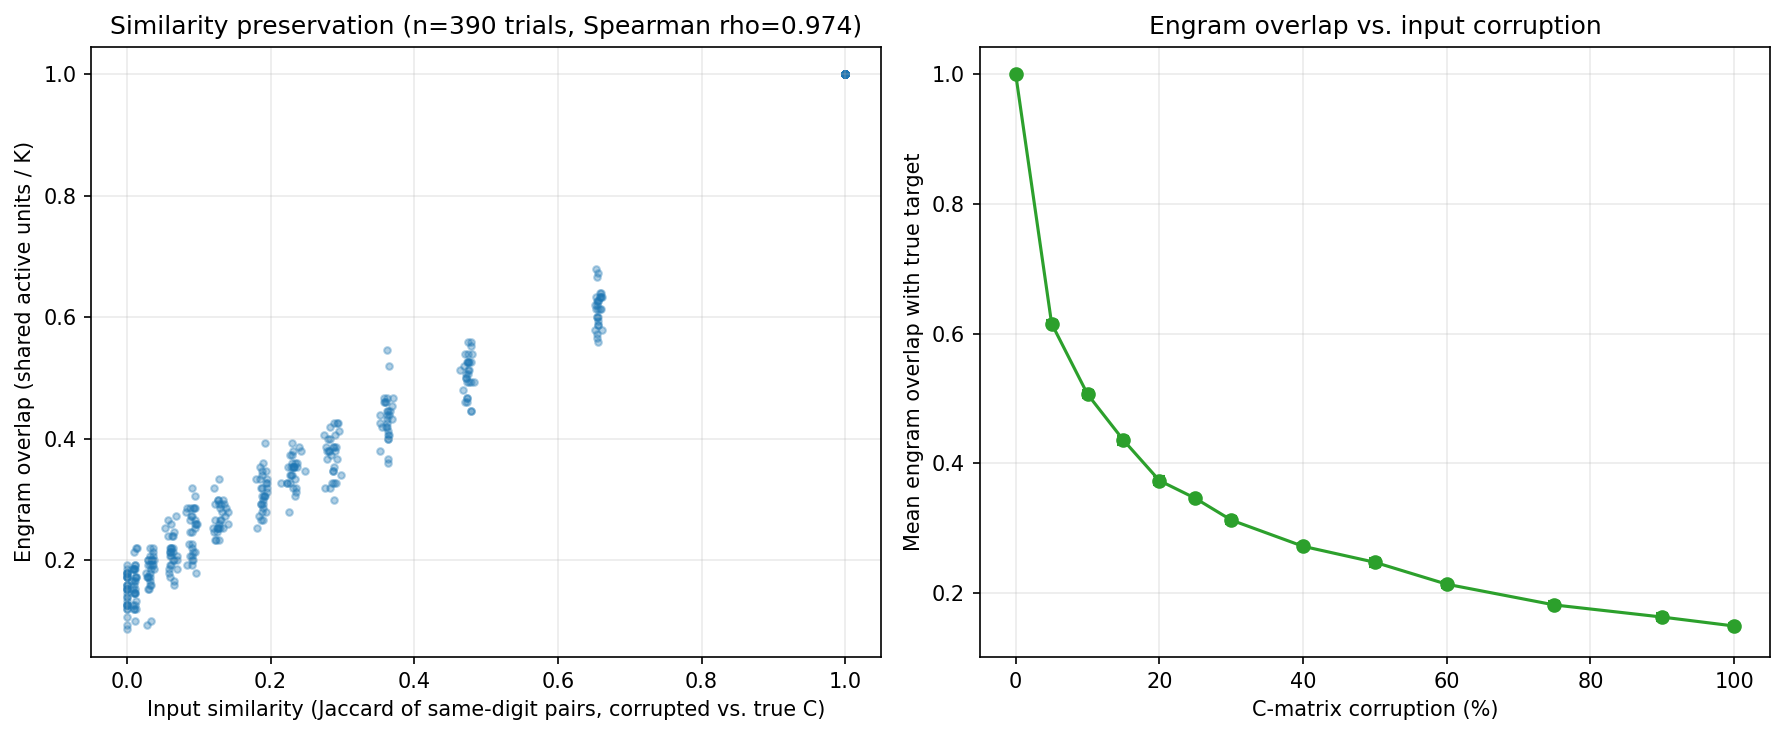
\includegraphics[width=\linewidth]{figures/hash_similarity_preservation.png}
\end{center}
\refstepcounter{figure}\label{fig:hashing}
\noindent\textbf{Figure \thefigure.} Left: engram overlap vs.\ input (coincidence-matrix)
similarity, pooled across all $13$ corruption levels and all $30$ target grids ($n=390$).
Right: mean engram overlap with the true target vs.\ percent corruption of the input
coincidence matrix (error bars: standard error across the $30$ targets at each level).

This result matters beyond confirming an analogy. A similarity-preserving encoder is exactly
what a downstream content-addressable readout needs in order to degrade gracefully rather than
catastrophically under query noise: if two inputs that are $90\%$ similar could map to
completely uncorrelated codes, no readout built on top of the code could recover a graceful
noise-tolerance curve, however good the readout's own separation mechanism is. The next
section holds this encoder fixed and asks how much of the resulting system's robustness comes
from the readout side.

\subsection{Separation operators: gap-based vs.\ ratio-based sharpening}
\label{sec:separation}

Gershman, Fiete \& Irie \cite{gershman2025} note that softmax, a hard top-$j$ threshold, and a
rectified-power nonlinearity are, respectively, the separation operators of Transformer-style
attention, sparse distributed memory \cite{kanerva1988}, and dense associative memory
\cite{krotov2016,ramsauer2020} -- three architectures differing only in this one nonlinearity,
alongside plain (identity) correlation-matrix memory \cite{kohonen1972}, which applies no
separation at all. We test this unification directly on the encoder characterized above: using
the same fixed $W_{SH}$ and the same $M=200$ stored engrams as
Section~\ref{sec:hashing}, we corrupt each query by flipping a swept fraction of its engram
bits, decode digit-cell values from $\hat b$ for each of six separation operators evaluated on
the identical corrupted queries at every noise level (a fully paired design, $100$ trials per
noise level, no error-correction cleanup pass, so as to isolate each operator's own behavior
rather than a downstream correction mechanism's).

\begin{center}
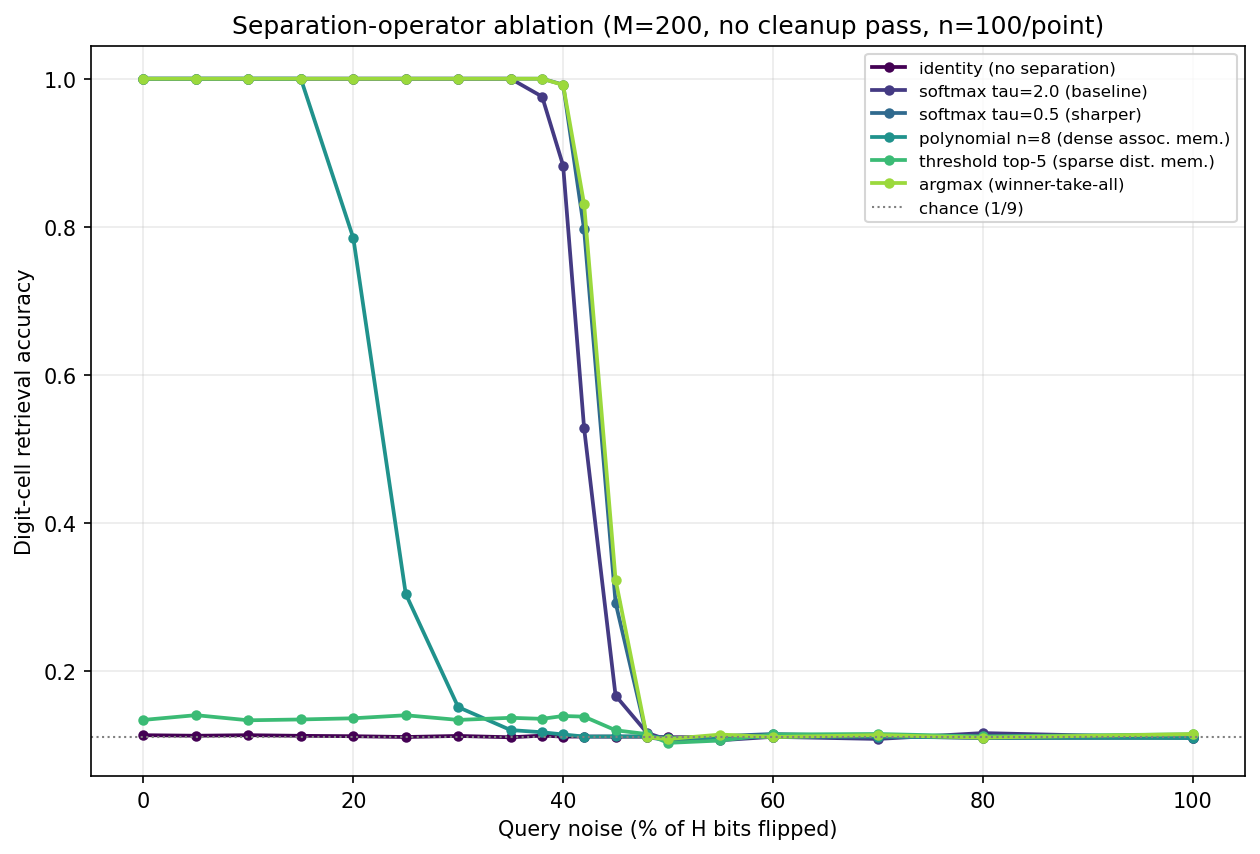
\includegraphics[width=0.85\linewidth]{figures/separation_operator_ablation.png}
\end{center}
\refstepcounter{figure}\label{fig:separation}
\noindent\textbf{Figure \thefigure.} Digit-cell retrieval accuracy vs.\ query noise for six
separation operators, evaluated on identical corrupted queries at every noise level
($M{=}200$, $n{=}100$/point, no cleanup pass).

Two findings depart from the intuition that a separation operator's robustness is set by how
aggressively it discriminates (``sharp separation is powerful but fragile''
\cite{gershman2025}). First, identity separation -- no nonlinearity at all -- performs at
chance \emph{even with a perfectly clean query} ($11.4\%$ vs.\ $100\%$ for softmax at $0\%$
noise): with $M{=}200$ competing memories, a linear reweighting cannot overcome the combined
pull of the other $199$ stored values on the weighted average, so some separating nonlinearity
is not merely a robustness refinement here but a strict requirement for retrieval to function
at all. Second, and more surprisingly, sharper is not uniformly more fragile: a hard-threshold
top-$5$ average (naively implementing sparse distributed memory's equal-weight readout) is
\emph{also} near chance at every noise level, including zero, because averaging five
equally-weighted stored values -- one correct, four spurious -- dilutes the correct digit
rather than recovering it, unlike real sparse distributed memory's per-bit majority vote over
redundant patterns. Meanwhile argmax (winner-take-all, the ``ideal noiseless'' operator
\cite{gershman2025}) and a sharpened softmax ($\tau=0.5$) hold up \emph{at least as well as}
the baseline softmax ($\tau=2.0$) right up to a shared collapse near $45$--$48\%$ noise --
sharpness itself is not the fault line.

The real fault line is gap-based vs.\ ratio-based sharpening. The rectified-polynomial
operator (dense-associative-memory-style, exponent $n=8$) collapses far earlier, around
$20$--$25\%$ noise, despite normalized zero-noise selectivity comparable to the other sharp
operators. We traced this mechanistically, with a dedicated exhaustive calculation over all
$M=200$ stored items (Table~\ref{tab:ratio}): even at zero noise, the best-competing wrong
memory already reaches, on average, similarity within a factor of $3.39$ of the true match's --
an extreme-value effect of having $199$ competitors, well below the naive factor of $6.67$
predicted from the mean chance-overlap floor alone ($H/K$) -- and this ratio shrinks toward $1$
as query noise grows.

\refstepcounter{table}\label{tab:ratio}
\noindent\textbf{Table \thetable.} Mean competitor ratio (true-match similarity / best-wrong-match
similarity), exhaustive over all $M{=}200$ stored items, vs.\ query noise.
\begin{center}
\begin{tabular}{lccc}
\toprule
Query noise & $0\%$ & $20\%$ & $30\%$ \\
\midrule
Mean competitor ratio & $3.39$ & $1.92$ & $1.45$ \\
\bottomrule
\end{tabular}
\end{center}
\noindent(Naive factor from the mean chance-overlap floor alone, $H/K$: $6.67$.)

A power of a ratio shrinking toward $1$ loses discriminative weight far faster than an
exponential of the corresponding absolute gap does, for the same starting margin --
softmax's exponential-of-a-gap form is intrinsically more robust than a power-of-a-ratio form
once a sizable number of competing memories guarantees a non-negligible interference floor.
This is a refinement, not a contradiction, of the unification in \cite{gershman2025}: the four
architectures are indeed the same computation with a different nonlinearity plugged in, but
which nonlinearity is the right engineering choice depends on the similarity statistics of the
memory system it operates over -- specifically, how many competing memories are stored and how
much residual similarity they carry -- not on sharpness alone.

\section{Discussion}

Taken together, these two results characterize both halves of a hippocampal-style key-value
memory -- the encoder and the readout -- on the same implemented system, rather than testing
either theoretical claim in isolation. Section~\ref{sec:hashing} shows that the encoder half
genuinely earns its analogy to the fly olfactory hashing circuit: it is not merely sparse and
combinatorial, but approximately similarity-preserving, the specific geometric property a
content-addressable readout depends on. Section~\ref{sec:separation} shows that the readout
half genuinely instantiates the unification proposed by \cite{gershman2025} -- the same stored
engrams and the same encoder support correlation-matrix-memory-style, sparse-distributed-memory-
style, dense-associative-memory-style, and Transformer-attention-style retrieval simply by
swapping one nonlinearity -- while also sharpening that theory's own stated intuition. The
theory's framing (sharper separation trades robustness for precision) predicts a single
ordered axis; what we find instead is two families that do not order along that axis at all:
gap-based operators (softmax at either temperature, argmax) remain close to tied with each
other regardless of sharpness, while the one ratio-based operator tested (rectified power)
collapses at roughly half their noise tolerance despite comparable zero-noise selectivity. The
mechanism we identify -- an extreme-value competitor-ratio calculation over $M-1$ stored
memories -- is a property of \emph{any} memory system with enough stored items to guarantee a
non-negligible interference floor, not an artifact of the Sudoku testbed, so we expect the same
gap-vs-ratio distinction to reproduce in other implementations of this same operator family.

A natural question is whether the two results are related beyond sharing an experimental
platform: does a similarity-preserving encoder make ratio-based sharpening fail sooner, or is
this purely a readout-side effect? Our design cannot separate these because both experiments
share the identical encoder; testing whether the gap-vs-ratio distinction depends on the
encoder's similarity-preservation would require deliberately degrading that property (e.g.\ by
adding an explicit decorrelating nonlinearity to $W_{SH}$'s output before $k$-WTA) and
re-running the separation-operator sweep on the degraded code -- a direct extension of this
work that we have not pursued here.

\section{Methods}

\textbf{Encoder.} $H=1000$, $K=150$ (density $\rho_K = K/H = 0.15$), fixed random projection
density $\rho=0.02$, nonzero entries i.i.d.\ $\mathcal{N}(0,1)$. Both experiments use the
identical fixed $W_{SH}$ and the identical pool of $M=200$ stored Sudoku grids (same random
seed for grid generation, projection, and engram construction).

\textbf{Section~\ref{sec:hashing} (hash test).} $30$ grids sampled without replacement from the
$M=200$ pool. Corruption: symmetric bit flips on the coincidence matrix's off-diagonal
same-digit entries, at fractions $\{0, 5, 10, 15, 20, 25, 30, 40, 50, 60, 75, 90, 100\}\%$ of
all $\binom{81}{2}$ cell pairs, independently sampled per trial. Input similarity: Jaccard
overlap of the same-digit pair sets between corrupted and true coincidence matrices. Engram
similarity: shared active units between corrupted and true engrams, divided by $K$. Statistic:
Spearman rank correlation, pooled across all $30\times13=390$ (target, corruption-level) pairs.

\textbf{Section~\ref{sec:separation} (separation-operator ablation).} Query corruption: a swept
fraction of the $H=1000$ engram bits flipped uniformly at random (independent draw per trial).
Six separation operators evaluated on identical corrupted queries at every noise level:
identity (no separation), softmax at $\tau=2.0$ (reference) and $\tau=0.5$ (sharpened), argmax
(winner-take-all), hard top-$5$ uniform average, and rectified power (exponent $n=8$,
normalized by $K$). No conflict-mask cleanup pass is applied, isolating each operator's raw
behavior. $100$ trials per noise level per operator, identical corrupted queries reused across
operators within a trial (paired design). The competitor-ratio calculation
(Table~\ref{tab:ratio}) is exhaustive rather than sampled: for each of the $M=200$ stored
items and each of three noise levels, the true-match similarity and the maximum similarity
among the other $199$ stored items are computed directly and averaged.

\section*{Code and Data Availability}
All simulation code, raw data (CSV), and figure-generation scripts are available at
\url{https://\allowbreak github.com/\allowbreak ghub-\allowbreak res1578/\allowbreak sudoku-\allowbreak hippocampal-\allowbreak key-\allowbreak value-\allowbreak memory}. This paper draws
specifically on \texttt{hash\_similarity\_preservation.py} (Section~\ref{sec:hashing}),
\texttt{separation\_operator\_ablation.py} (Section~\ref{sec:separation}),
\texttt{separation\_operator\_competitor\_ratio.py} (Table~\ref{tab:ratio}), and the shared
core module \texttt{hippocampus\_drive\_readout.py} that both scripts import the encoder and
stored engram pool from. The repository's README gives exact commands to regenerate every
number, table, and figure above.

\bibliographystyle{plain}
\begin{thebibliography}{99}

\bibitem{marr1971} D.~Marr, ``Simple memory: a theory for archicortex,''
\textit{Phil.\ Trans.\ R.\ Soc.\ Lond.\ B} \textbf{262}, 23--81 (1971).

\bibitem{rolls2013} E.~T.~Rolls, ``The mechanisms for pattern completion and pattern
separation in the hippocampus,'' \textit{Front.\ Syst.\ Neurosci.}\ \textbf{7}, 74 (2013).

\bibitem{hopfield1982} J.~J.~Hopfield, ``Neural networks and physical systems with emergent
collective computational abilities,'' \textit{PNAS} \textbf{79}, 2554--2558 (1982).

\bibitem{willshaw1969} D.~J.~Willshaw, O.~P.~Buneman, H.~C.~Longuet-Higgins, ``Non-holographic
associative memory,'' \textit{Nature} \textbf{222}, 960--962 (1969).

\bibitem{krotov2016} D.~Krotov, J.~J.~Hopfield, ``Dense associative memory for pattern
recognition,'' \textit{NeurIPS} (2016).

\bibitem{ramsauer2020} H.~Ramsauer et al., ``Hopfield networks is all you need,''
\textit{arXiv:2008.02217} (2020).

\bibitem{gershman2025} S.~J.~Gershman, I.~Fiete, K.~Irie, ``Key-value memory in the brain,''
\textit{Neuron} \textbf{113}, 1694--1707 (2025).

\bibitem{kohonen1972} T.~Kohonen, ``Correlation matrix memories,'' \textit{IEEE Trans.\
Comput.} \textbf{C-21}, 353--359 (1972).

\bibitem{kanerva1988} P.~Kanerva, \textit{Sparse Distributed Memory}, MIT Press (1988).

\bibitem{vaswani2017} A.~Vaswani, N.~Shazeer, N.~Parmar, J.~Uszkoreit, L.~Jones,
A.~N.~Gomez, L.~Kaiser, I.~Polosukhin, ``Attention is all you need,'' \textit{NeurIPS}
\textbf{30} (2017).

\bibitem{schlag2021} I.~Schlag, K.~Irie, J.~Schmidhuber, ``Linear Transformers Are Secretly
Fast Weight Programmers,'' \textit{ICML} (2021).

\bibitem{dasgupta2017} S.~Dasgupta, C.~F.~Stevens, S.~Navlakha, ``A neural algorithm for a
fundamental computing problem,'' \textit{Science} \textbf{358}, 793--796 (2017).

\end{thebibliography}
\end{document}
